\chapter{Motions}
\label{chap:Motions}
\begin{figure}[H]
    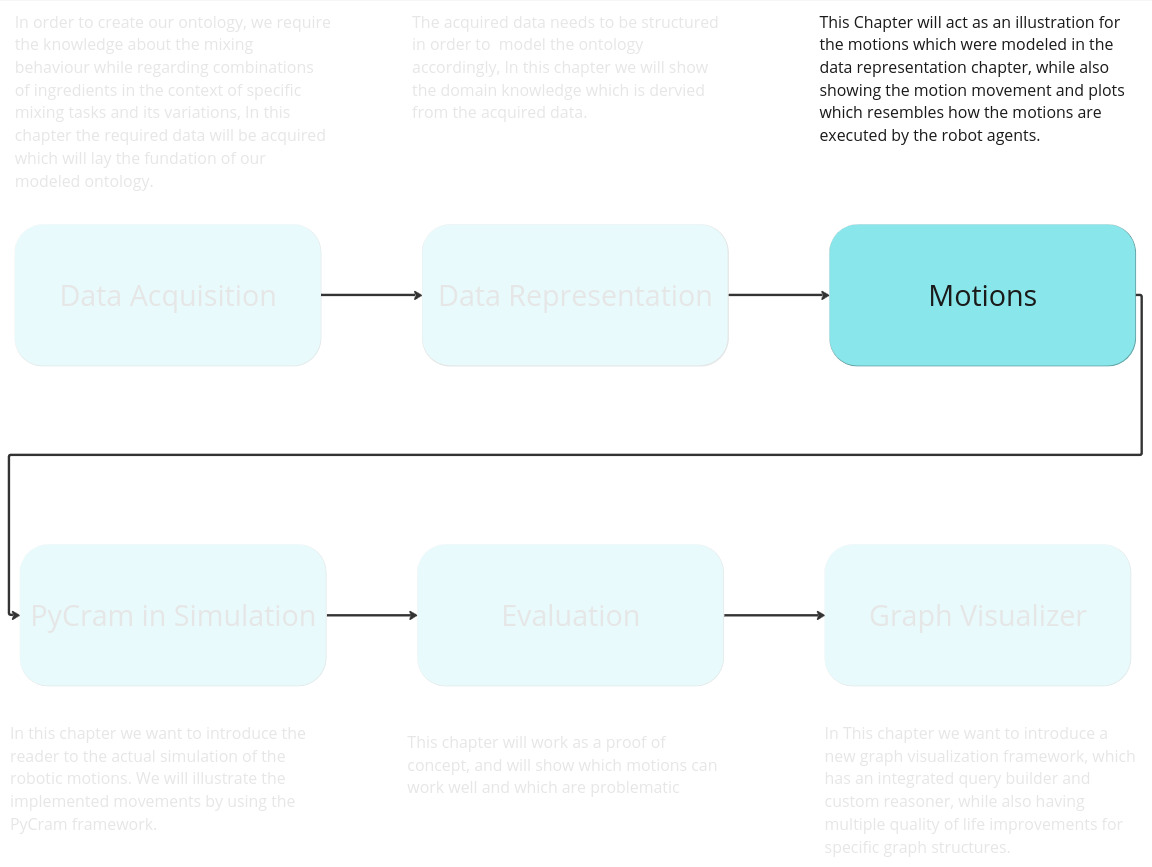
\includegraphics[scale=0.3]{Graphics/overview_3.jpg}
\end{figure}
In this chapter we'll describe on an abstract level how the motions are implemented in pycram2.
To simplify the implementation of motions, we hold the following assumptions about the motions which are performed on containers.
Firstly we assume, the container is symmetric in the x,y direction. We don't consider the descent of the container, we keep the height for the tool
constant over the performed motion. We don't have collision detection.

\section{Circular Motion}
The circular motion is generated on a circular plane. 
By having a center coordinate = $(x,y)$, which is the center coordinate of 
the container to execute the Circular Motion, we generate a set of coordinates
with the following functions: 

$circleX = containerCenterX + radius * cos(radian)$

$circleY = containerCenterY + radius * sin(radian)$

We retrieve the respective radians using the following function:

$ angle2radian = angle * \frac{\pi}{180} $

Here, we pick a sequence of angles starting from
0 to 360 degrees convert these into radians in order to generate points lying on a circle.

INSERT Plot

\section{Folding Motion}
The folding motion is not a circular motion but rather a linear motion. In its current implementation, the motion is a singular line having where one endpoint is on the edge of the container
the other is center of the container. While the motion in itself is a straight line going through the container, the motion is executed by traversing from one end of the container to the center,
and then repeating the motion flipped - from center to one of the end, which creates a folding effect.
This line partially covers the whole container, therefore the direction has to be realigned in order to mix different sections of the container.

By constructing a 2D rotation matrix for some angle, where the angle determines the shift of the line $\theta$:
\[R(\theta) = \begin{bmatrix}
    \cos(\theta) & -\sin(\theta) \\
    \sin(\theta) & \cos(\theta)
     \end{bmatrix}
 \] 

a transformation onto the line can be applied, which shifts the line using this function: 

$\begin{bmatrix} x' \\ y' \end{bmatrix} = R(\theta) * \begin{bmatrix} x \\ y \end{bmatrix}$

The folding motion is executed multiple times, in that the motion is covering multiple parts of the container, depending on what 
the value of the angle is to shift the folding line. 

Once the folding motion has finished, by shifting the folding line another time with an angle $\phi$
we realign the line, so that different parts of the container can be folded by using angle $\theta$ again.

INSERT Plot

\section{Horizontal Elliptic Motion}
The horizontal elliptic motion is executed on a horizontal plane and involves multiple ellipses.
Using the function to compute x,y coordinates on a circle, we use one constant radius and one radius which is changing. 

By using the formular to compute points on a circle, we adjust the radius for 
x,y, where one of the values is set to 0.01, the other one is sampled evenly from the interval $semi\_major\_radius = (radius\_upper\_bound,radius\_upper\_bound / 2 ).$
We take the maximum sampled radius which fulfills the following condition. 
$\sqrt{(x\_{i} - center\_x)^2 + (y\_{i} - center\_y)^2} < radius_upper_bound$
Additionally we decrement and increment y coordinates. If the condition: $\sqrt{(y\_{i} - center\_y)^2} > radius_upper_bound$
is met we change from decrementing to incrementing and vice versa until this condition is fulfilled again.

\section{Whirlstorm Motion}
The whirlstorm motion uses the function to generate points lying inside a circle, with differing radiuses, over the course of the motion. 
Using an upper bound radius and a lower bound radius, we create an evenly spaced interval between those radiuses, to use them for coordinate generation. 
Starting from the upper bound to the lower bound translates to performing the motion from the edge to the center or close to the center, depending on the 
values of upper and lower bound radius. 

To create a consistent and fluid motion, we introduce mirroring of the coordinates and alternating from outer to inner circular motion and vice versa.
These are visualized in these plots:


